\documentclass[12pt]{article}

\usepackage[a4paper]{geometry}
\usepackage[warn]{mathtext}
\usepackage[T2A]{fontenc}
\usepackage[utf8]{inputenc}
\usepackage[russian,english]{babel}
\usepackage{amssymb,amsmath}
\usepackage{hyperref}
\usepackage{indentfirst}
\usepackage{listings}
\usepackage{graphicx}
\usepackage{subfig}
\usepackage[export]{adjustbox}

\renewcommand*\contentsname{Contents (detailed)}

% \usepackage{rumathbr}
% \usepackage{std}

% \widowpenalty=500
% \clubpenalty=500

\begin{document}

    \title{\textbf{Coursework report}}
    \author{Goncharov Vladimir}

    \thispagestyle{empty}

    \begin{center}
    ~\\[10ex]
    {National Research University ``Higher School of Economics''}\\[1.1ex]
    Faculty of Computer Science\\[1.1ex]
    Applied mathematics and informatics\\[15.0ex]
    {\LARGE\bf Coursework report}\\[4.0ex]
    {\Large\bf Implement autonomous navigation system for quadcopter capable of tracking clearly marked objects}\\[4.0ex]
    student: Vladimir Goncharov\\
    research advisor: Bruno Bauwens\\[4.0ex]
    2016
    \end{center}

    \newpage

    \thispagestyle{empty}

    % \pdfbookmark[1]{Contents}{toc}
    % \shorttoc{Contents}{1}

    \tableofcontents

    \newpage

    \setcounter{page}{1}

    \section{Introduction}

    The goal of this project is to implement a relatively simple
    well documented control system for ARdrone 2 quadcopter
    capable of tracking a special mark (that is, a flat object that is known
    before launch).
    Using drone's bottom camera to find a target, the application generates
    and sends commands to the drone so that it hovers above the target.

    The purpose of the work is not to bring a new control or computer vision
    algorithm but to provide a solid software base for further work
    with the drone. The creation of any robotic control system requires
    implementation of the supporting components, such as
    the debug system, the user interface, and hardware drivers
    are necessary to control any robot.

    The idea is that these components are made reusable so that they
    can be plugged in to any project without much adaptation. That is, the
    code of the application that is presented in this work can be used as
    a base for any project that requires controlling the ARdrone 2
    quadcopter.

    The control structures, such as the user interface and
    the drone control system, are presented in this paper along with the
    target recognition algorithm.


    \section{Technologies~overview}

    Robot Operating System (ROS) package is used as a main framework.
    ROS is an open-source C++ library for implementing efficient modular
    distributed yet simple systems. It comes with many useful
    features which makes the development easier.

    To communicate with the drone, the ``ArdroneAuthonomy''
    package is used~\cite{ArdroneAuthonomy}.
    This package is built on top of ROS. It provides simple interface for
    the drone's manipulation.

    For image processing, an open-source computer vision library called OpenCV is used.

    For interface rendering, another open-source library called QT is used.
    
    To work with the drone, I'm using Python programming language.
    It provides the ability to rapidly develop big systems while maintaining
    overall simplicity. Python code is easier to read and easier to write.

    ROS and OpenCV are written in C++. However, Python programming language
    bindings are available for both of them.

    It is necessary to note that Pythonå
    was developed to be used in the IO-bound systems.
    Those systems spend more time waiting for user input rather than calculating.
    However, almost all robot control algorithms are real-time and CPU-bound.
    They spend most of the time calculating the result rather than waiting.

    This fact makes Python less applicable for the robotic projects.
    For the bigger systems, C++ programming language may be the better choice.
    
    Note also thet it is possible to combine Python and C++ to acheve flexibility,
    computational efficiency, and simplicity at the same time.


    \subsection{ARDrone}

    As a hardware platform, the ``Parrot'' ARDrone 2 is used.
    It is a light quadcopter that has a number of advantages,
    including simplicity of control. Also, it is strong enough to
    withstand falls from sufficient height, which is good for testing
    a software.

    ARDrone has two on-board cameras along with accelerometers, gyroscopes,
    altimeter, and other sensors.

    In this project, the bottom camera is used for controlling the drone.
    However, it turns out that this camera is not the best choice.
    It has lower resolution than the front camera, the image is blurred.
    But the most important thing is that is has small field of view.
    This makes the algorithm not as stable as it could be.

    \subsection{Environment}

    To run the project, ROS version ``Jade'' is used. The project should also work with
    the newer version of ROS called ``Kinetic Kame''. It wasn't
    tested with this version, though.

    Using ROS imposes some restrictions.
    Ubuntu operating system is required to run the code.
    There is also a beta release of ROS for OSX.

    To make development process easier, it is
    possible to use virtualization systems, such as VirtualBox.

    Remember, however, that these systems should be used with caution.
    They can cut off the GPU support which will decrease speed of
    image processing.

    \subsection{ROS~and~ArdroneAuthonomy}

    As it was mentioned before, ROS allows easy implementation
    of distributed systems.

    The key to the simplicity is ``modularity'' approach.
    Any ROS application consists of a set of many separate executables
    called ``nodes''~\cite{ROSsite}. Each node is a simple program
    that can be written in either C++ or Python.

    Nodes are connected into a single network.
    They communicate by sending messages
    through the ROS master server and by listening for messages
    from the other nodes.

    Messages are grouped into
    channels called ``topics''~\cite{rostopic}.
    Each topic contains messages of a particular type.
    Each node can publish a message to any topic and each node can subscribe
    to any topic to listen for messages and process them.

    For example, there is a user interface (UI) node in the project which shows a video
    stream as transmitted by another node. The implementation of another node
    is unknown for the UI node. Thus, it can work with any node that can publish
    a video. The interface can be setted up to work with the drone's front camera,
    bottom camera, or any other video stream. Neither setup requires changing
    the interface node itself~--- it's enough to reroute messages from any
    node to the UI node.

    Figure \ref{fig:reroute} shows how the video stream
    flows through the system. From the drone it gets to the processing node
    and than to the UI node.
    Note that nodes are using local topic names. For each node it is possible
    to remap names of topics so that nodes can use any convenient names
    without care for global names.

    \begin{figure}[htbp]
        \noindent\centering
            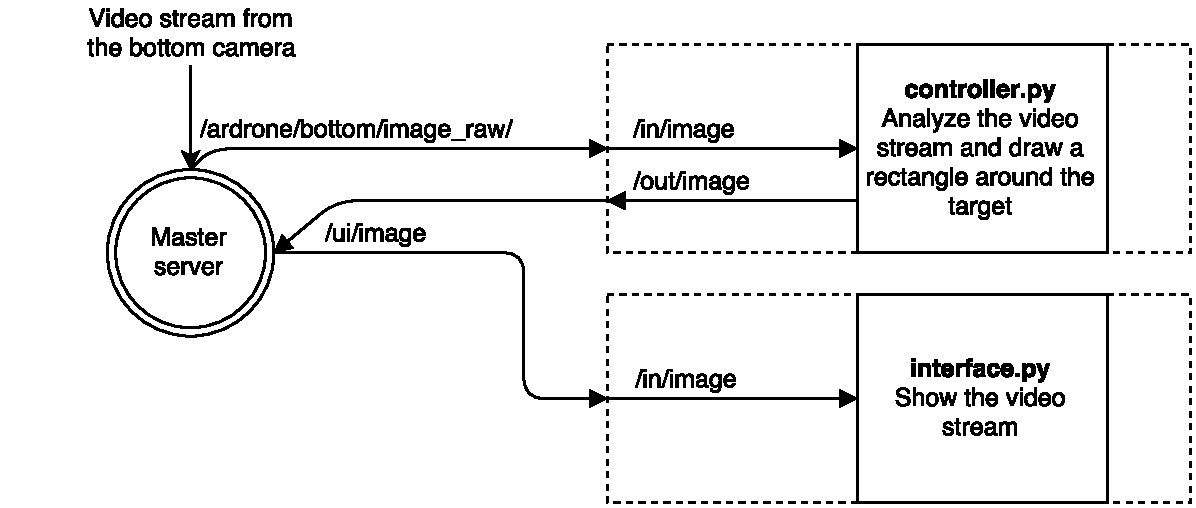
\includegraphics[width=\textwidth]{reroute.pdf}
        \caption{Rerouting video stream from the drone to the processing node
        and than to the UI node.}
        \label{fig:reroute}
    \end{figure}

    The ``ArdroneAuthonomy''~\cite{ArdroneAuthonomy}
    package provides nodes for communicating
    with the drone. Those nodes transmit several important data streams,
    such as the drone's status, its battery charge level, its sensors data,
    and so on.

    \subsection{OpenCV}
    
    OpenCV is a well-known computer vision library written in C++.
    Version 2.4 is used in this project as it comes as a dependency
    for the ROS install.

    OpenCV implements a lot of popular algorithms. Tools for target
    recognition process~\cite{SURF, ORB}, camera calibration~\cite{OpenCVCalib},
    and estimating 3d coordinates of the detected object~\cite{OpenCV3dRec}
    are included.

    Note that using OpenCV with Python adds some limitations to your program.
    Python bindings for OpenCV 2.x doesn't allow use of several important
    features, such as the Kalman filter. Python bindings for OpenCV 3.x contain
    bugs leading to memory leaks. It would be preferanle to implement
    computer vision nodes in C++.

    \section{Project~structure~and~APIs}

    The project consists of two nodes and several classes.

    The structure is common for all ROS projects:

    \begin{itemize}
        \item {\bf launch/}~--- this directory contains xml files that
        are instructions on how to launch the system. See~\cite{roslaunch}
        for usage.
        \begin{itemize}
            \item autopilot.launch~--- launches the main program.
            \item environment.launch~--- launches the ArdroneAutonomy driver.
        \end{itemize}
        \item {\bf nodes/}~--- this directory contains the actual Python code.
        \begin{itemize}
            \item controller.py~--- contains the image analysis algorithms and
            the autopilot logic.
            \item interface.py~--- provides user interface.
            \item state\_logger.py~--- helper node, used to print out all
            changes of the drone's state.
            \item {\bf utils/}~--- contains reusable helper classes.
            \begin{itemize}
                \item drone.py~--- provides the DroneController class that is
                used to interact with the ArdroneAutonomy package.
                \item events.py~--- provides event support.
            \end{itemize}
        \end{itemize}
        \item package.xml~--- a description of the ROS package.
    \end{itemize}

    \subsection{Interface}
    \label{ssec:interface}

    The first node called ``interface.py''. It implements a QT interface for
    controlling the drone. This node provides view of the video from the drone's
    camera and keyboard control of the drone.

    \begin{figure}[htbp]
        \noindent\centering
            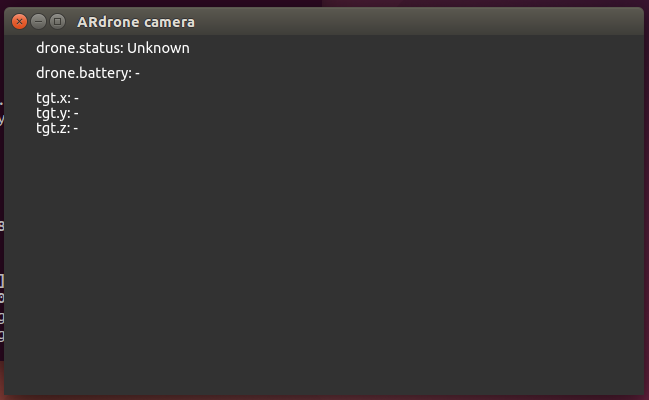
\includegraphics[width=.7\textwidth]{ui.png}
        \caption{View of the interface while the drone is offline.
        The debug messages are at the left side of the screen. The video stream
        is displayed behind them (the gray area).}
        \label{fig:ui}
    \end{figure}

    It also provides the ability to display debug messages. A special text
    topic called ``/ui/message'' can be used to send any text to this node.
    The node will display the text based on its structure.
    
    Those messages formed like ``name::messsage'' will update information
    on the left side of the screen (figure~\ref{fig:ui}). That is, sending ``tgt.x::10'' will make
    the ui node to show the value of 10 near the ``tgt.x'' caption.

    Messages which doesn't match the above pattern will be shown on the right
    side of screen. They will be displayed for ``message\_display\_time'' time
    (which is 5sec. by default) and then removed from the screen.

    The node listen for three topics:

    \begin{itemize}
        \item {\bf /ardrone/navdata}~--- information about the drone state.
        \item {\bf /in/image}~--- video stream to be displayed.
        \item {\bf /ui/message}~--- messages stream.
    \end{itemize}

    Keyboard controls are configurable. By default, `WSADQE' are used to
    control drone's speed, `[' and `]' are used to
    control drone's altitude, `T' for takeoff, `L' for land, `R' for emergency
    stop/reset, `Y' to activate/deactivate the control algorithm.

    \subsection{Controller}

    The controller node is the place where the main code runs.
    The code and the algorithm itself are described in the further sections.
    It consists of two parts. The first one detects the target
    on the video stream (see section~\ref{sec:target_recognition_algorithm}).
    The second one estimates the position of the target relative to the drone
    and generates commands (see section~\ref{sec:drone_control_algorithm}).

    The controller can be activated and deactivated by hitting the `Y'
    key while the interface is active.

    If this node is active, keyboard controls are disabled, except for the
    landing, reset, and controller toggle keys.

    \subsection{Classes~and~utilities}

    Here comes a description of the reusable classes used in this project.

    Basically, each node contains a main class that implements its behaviour
    so that it can become a base for another node.
    However, there are several additional classes in the `utils/'
    directory.

    All class relations can be observed in figure~\ref{fig:uml}.

    \begin{figure}[htbp]
        \noindent\centering
            \includegraphics[width=\textwidth]{uml.pdf}
        \caption{Class diagram.}
        \label{fig:uml}
    \end{figure}

    \paragraph{Interface} The interface node is designed to be reusable.
    It consists of two classes: ``Messages'' and ``UInode''.

    The first one is here to store the debug messages and to display them.
    For temporary messages (see~\ref{ssec:interface}), there is a queue
    of them. For the permanent ones, there is a structure which describes
    how to display those messages.

    Here is an example of that structure which output is shown in figure~\ref{fig:ui}:

    \begin{lstlisting}[frame=single,language=Python]

grid = [
    # Name of the message.
    'drone.status',

    # None creates a little gap between two messages
    # so you can visually split them into groups.
    None,

    'drone.battery',
    
    None,
    
    'tgt.x',
    'tgt.y',
    'tgt.z',
]

    \end{lstlisting}

    The second class is the interface node itself.
    It is derived from the ``QtGui.QMainWindow''. You can extend
    its functionality by creating a node derived from this class.

    % TODO docs

    \paragraph{DroneController} To interact with the ArdroneAutonomy,
    there is a ``DroneController'' class along with two helpers: ``Event''
    and ``DroneStatus''.

    The ``DroneStatus'' class represents drone's state
    as received from the drone.
    It can convert a status code to a human-readable string.

    The drone sends a numerical code that represents its state.
    I haven't been able to find a reliable description of them so I've
    made a list of all possible states:

    \begin{itemize}

        \item {\bf0: emergency}~--- This is set after the ``reset'' command
        or a failure.
        This state is also set by the driver when it
        loses the connection to the drone. I'd not perform any actions on this state.

        \item {\bf1: initialized}~--- A wired one. I've never seen this state actually set.

        \item {\bf2: landed}~--- The drone is on the ground.

        \item {\bf3: flying}~--- The drone is flying. Its velocity is non-zero.

        \item {\bf4: hovering}~--- The drone is hovering, e.g. its trying to keep its position constant.

        \item {\bf5: test}~--- No idea what it is.

        \item {\bf6: unconnected}~--- Different guides says different things about this state.
        I've never seen this state actually set. So better don't use it.

        \item {\bf7: taking off}~--- This state is set after the drone receives the ``takeoff'' command.
        However, the official documentation calls this state
        ``going to hover mode'' without any explanation.

        \item {\bf8: going to hover mode}~--- This state is set after the drone receives the ``hover'' command.
        However, the official documentation calls this state
        ``landing'' without any explanation.

        \item {\bf9: looping}~--- This state is set when the drone is going to land.
        It's probably set when the drone executes an animation.
        Never tested it, though.

        \item {\bf-1: unknown}~--- The drone is offline. This state is set
        by the `DroneController` class. You can't receive negative values
        from the drone itself.

    \end{itemize}

    The ``Event'' class is a simple event dispatcher. It stires callbacks
    and runs them whenever the event is triggered.

    The ``DroneController'' class can be used to monitor the drone's status and
    to send commands to the drone. It also triggers events whenever
    the drone changes its state:

    \begin{itemize}

        \item {\bf on\_online}~--- executed whenever the drone gets on-line.
          This event will be emitted just after a new data received
          from the drone. This mean that you won't have any
          useful data in the ``DroneController'' instance at the moment.
          The drone state and other variables of the class
          will be populated after.
        \item {\bf on\_offline} -- executed whenever the drone gets offline.
            This event is emitted at last, after ``on\_state\_change'' and all
            other events.

        \item {\bf on\_status\_change}~--- executed whenever the drone changes its status.

        \item {\bf on\_status\_emergency}~--- executed whenever the drone
          changes its status to ``emergency''.
        \item {\bf on\_status\_initialized}~--- executed whenever the drone
          changes its status to ``initialized''.
        \item {\bf on\_status\_landed}~--- executed whenever the drone
          changes its status to ``landed''.
        \item {\bf on\_status\_flying}~--- executed whenever the drone
          changes its status to ``flying''.
        \item {\bf on\_status\_hovering}~--- executed whenever the drone
          changes its status to ``hovering''.
        \item {\bf on\_status\_test}~--- executed whenever the drone
          changes its status to ``test''.
        \item {\bf on\_status\_unconnected}~--- executed whenever the drone
          changes its status to ``unconnected''.
        \item {\bf on\_status\_taking\_off}~--- executed whenever the drone
          changes its status to ``taking\_off''.
        \item {\bf on\_status\_going\_to\_hover\_mode}~--- executed whenever the drone
          changes its status to ``going\_to\_hover\_mode''.
        \item {\bf on\_status\_looping}~--- executed whenever the drone
          changes its status to ``looping''.
        \item {\bf on\_status\_unknown}~--- executed whenever the drone
          changes its status to ``unknown''.

        \item {\bf before\_cmd\_takeoff}~--- executed whenever the ``takeoff'' command is sent
          to the drone.
        \item {\bf before\_cmd\_land}~--- executed whenever the ``land'' command is sent
          to the drone.
        \item {\bf before\_cmd\_reset}~--- executed whenever the ``reset'' command is sent
          to the drone.
        \item {\bf before\_cmd\_hover}~--- executed whenever the ``hover'' command is sent
          to the drone.
        \item {\bf before\_cmd\_vel}~--- executed whenever the ``vel'' command is sent
          to the drone.
        \item {\bf before\_cmd}~--- executed whenever new velocity message is sent
          to the drone.

    \end{itemize}

    See the ``state\_logger.py'' for usage of this events.

    ``DroneController'' contains API to control the state of the drone:

    \begin{itemize}
        \item {\bf takeoff()}~--- send the takeoff signal.
    
        \item {\bf land()}~--- send the land signal.
    
        \item {\bf reset(force)}~--- Send the reset signal.
        Warning: the reset signal causes immediate engine shutdown.
        Therefore the land signal is sent instead of reset while flying.
        Set ``force'' flag to cancel this behavior.

        \item {\bf hover()}~--- Send the hover signal.
        This will kill all velocities and enable the drone to auto-hover.

        \item {\bf send\_vel(x, y, z, yaw)}~--- Send new velocities to the drone.

        This method recovers previously sent command in order to
        keep values that are not provided (e.g. None).
        That is, executing

    \begin{lstlisting}[frame=single,language=Python]
controller.send_vel(x=1, y=0)
controller.send_vel(z=1)
    \end{lstlisting}

        is equvivalent to

    \begin{lstlisting}[frame=single,language=Python]
controller.send_vel(x=1, y=0, z=1)
    \end{lstlisting}

        Such behaviour can cause troubles in the multi-threaded environments.
        Thus, is better to set all parameters explicitly.

    \end{itemize}


    \subsection{Additional~components}

    There are also nodes and classes that are not in the class diagram.
    They are used as a base to create quick tests of a new functionality.

    \paragraph{nodes\_dev/base.py} This is the base for nodes that are
    actively interact with the OpenCV code. The idea is simple: if you want
    to test a new CV algorithm, you can just derive from the
    ``BaseStreamHandler'' and develop your OpenCV code without care for any
    other components. All interactions with ROS are implemented in this
    base class.

    \paragraph{frame.py} This node based on BaseStreamHandler.
    It is used to test accelerometers and gyroscopes. Based on the
    estimated drone's position, it projects a set
    of points onto the image so that those points look like being stuck to the floor.

    \paragraph{delay.py} This node based on BaseStreamHandler.
    It is used to test delays in the signal transmission.

    Place the drone before the screen of a computer. After the node
    is launched, it displays black and white rectangles. Once per second
    it changes the color of the rectangle from black to white
    and waits for the image transmitted by the drone to change its brightness.

    This way it is possible to measure the delay between an image is captured
    by the camera and this image received by the node.
    The delay is near 300ms.

    \paragraph{BaseStreamHandler example}
    As an example of usage of the ``BaseStreamHandler'' class, lets
    take a look at the ``delay.py'' implementation:

    \begin{lstlisting}[frame=single,language=Python]
import rospy
import cv2
import numpy as np
from datetime import datetime
from base import BaseStreamHandler


# Node is derived from the BaseStreamHandler
class DelayMesure(BaseStreamHandler):
    def __init__(self, *args, **kwargs):
        """Initialize the node"""
        
        # The `seek' flag becomes true
        # when the test is running.
        self.seek = False
        # Time when the color has been changed.
        self.time = None

        # Black and white rectangles.
        self.black = np.zeros((600, 800, 3), np.uint8)
        self.white = np.zeros((600, 800, 3), np.uint8)
        self.white[:, :] = (255, 255, 255)

        # Set up ROS to call the `self.run_test'
        # function once per second.
        rospy.Timer(rospy.Duration(1), self.run_test,
                    oneshot=False)

        # Initialize the `BaseStreamHandler'.
        super(DelayMesure, self).__init__(*args, **kwargs)

    def run_test(self, *args, **kwargs):
        """Run a new test"""
        # If the test is not running...
        if not self.seek:
            # Launch a new test!

            # Show the white image
            cv2.imshow('Test', self.white)
            cv2.cv.WaitKey(1)
            
            # Indicate that the the test is running
            self.seek = True

            # Set up current time
            self.time = datetime.now()

    def on_image(self, img):
        """Process images"""
        # This function gets called for each frame
        # in the video stream.

        # It the test is running and
        # overall brightness of the image is high enough...
        if self.seek and img.mean() > 100:
            # We've received a frame
            # with the white rectangle.

            # Print how long has it took
            # to transmit the image.
            print(datetime.now() - self.time)

            # Indicate that the the test is not running
            self.seek = False

            # Show the black image
            cv2.imshow('Test', self.black)
            cv2.cv.WaitKey(1)

        return img


if __name__ == "__main__":
    # All launching process is already implemented
    # in the `BaseStreamHandler'.
    # You don't have to worry
    # about launching the IO loop
    # or registering the node.
    # Just call the `launch_node()' function.
    DelayMesure.launch_node()
    \end{lstlisting}

    \subsection{Messages~flow}

    There are several topics through which messages are transmitted between nodes.
    Global structure can be found in figure~\ref{fig:topics}.

    \begin{figure}[htbp]
        \noindent\centering
            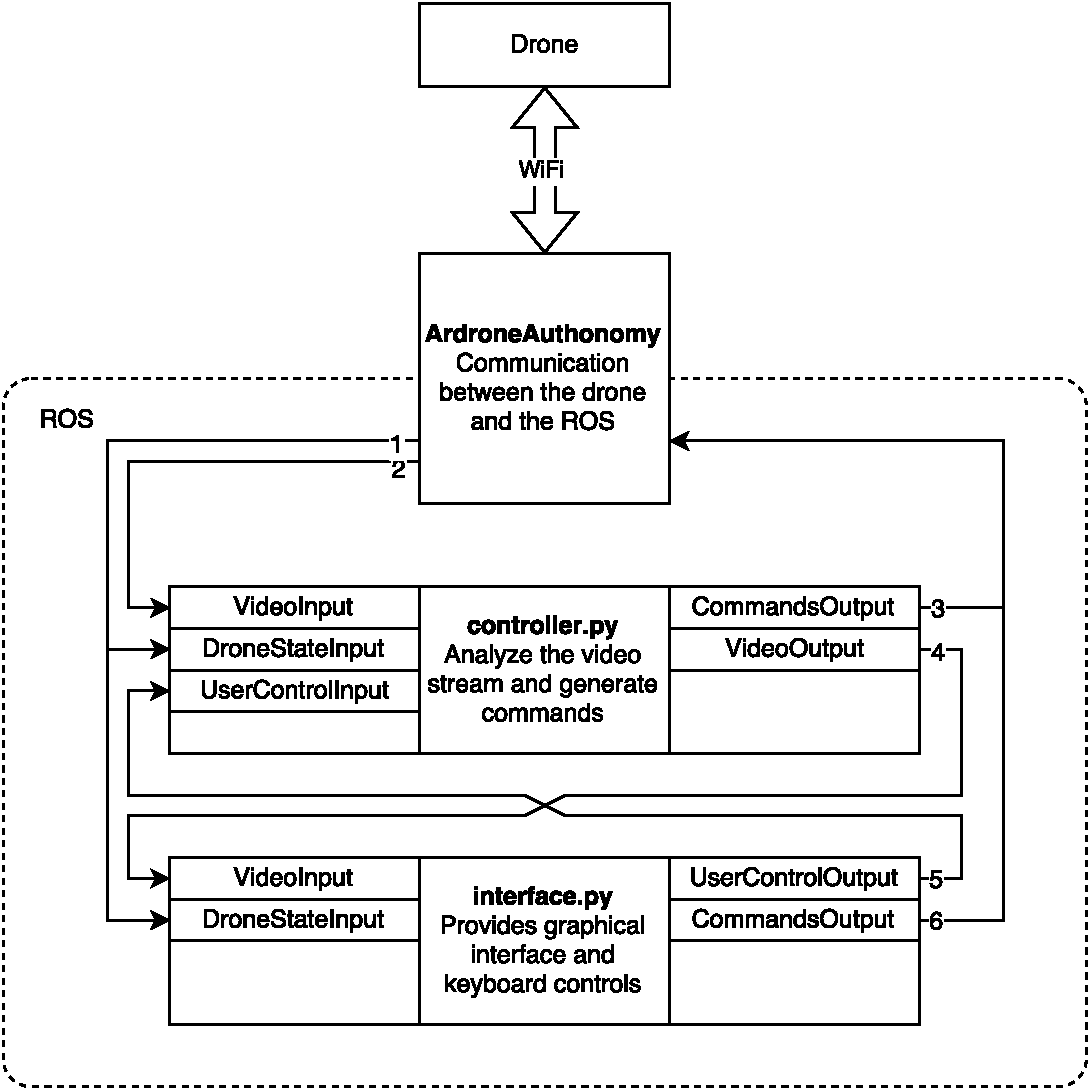
\includegraphics[width=\textwidth]{topics.pdf}
        \caption{Topics and messages flow.} % TODO something!!
        \label{fig:topics}
    \end{figure}

    \section{Target~recognition~algorithm}
    \label{sec:target_recognition_algorithm}

    The first part of the control application is the target recognition
    algorithm. Basically, there is an image of the target (I call it a true image),
    and I want to find that image in a video frame (figures~\ref{fig:target} a and b).

    \begin{figure}[htbp]
        \noindent\centering
        \subfloat[The target pattern]{
          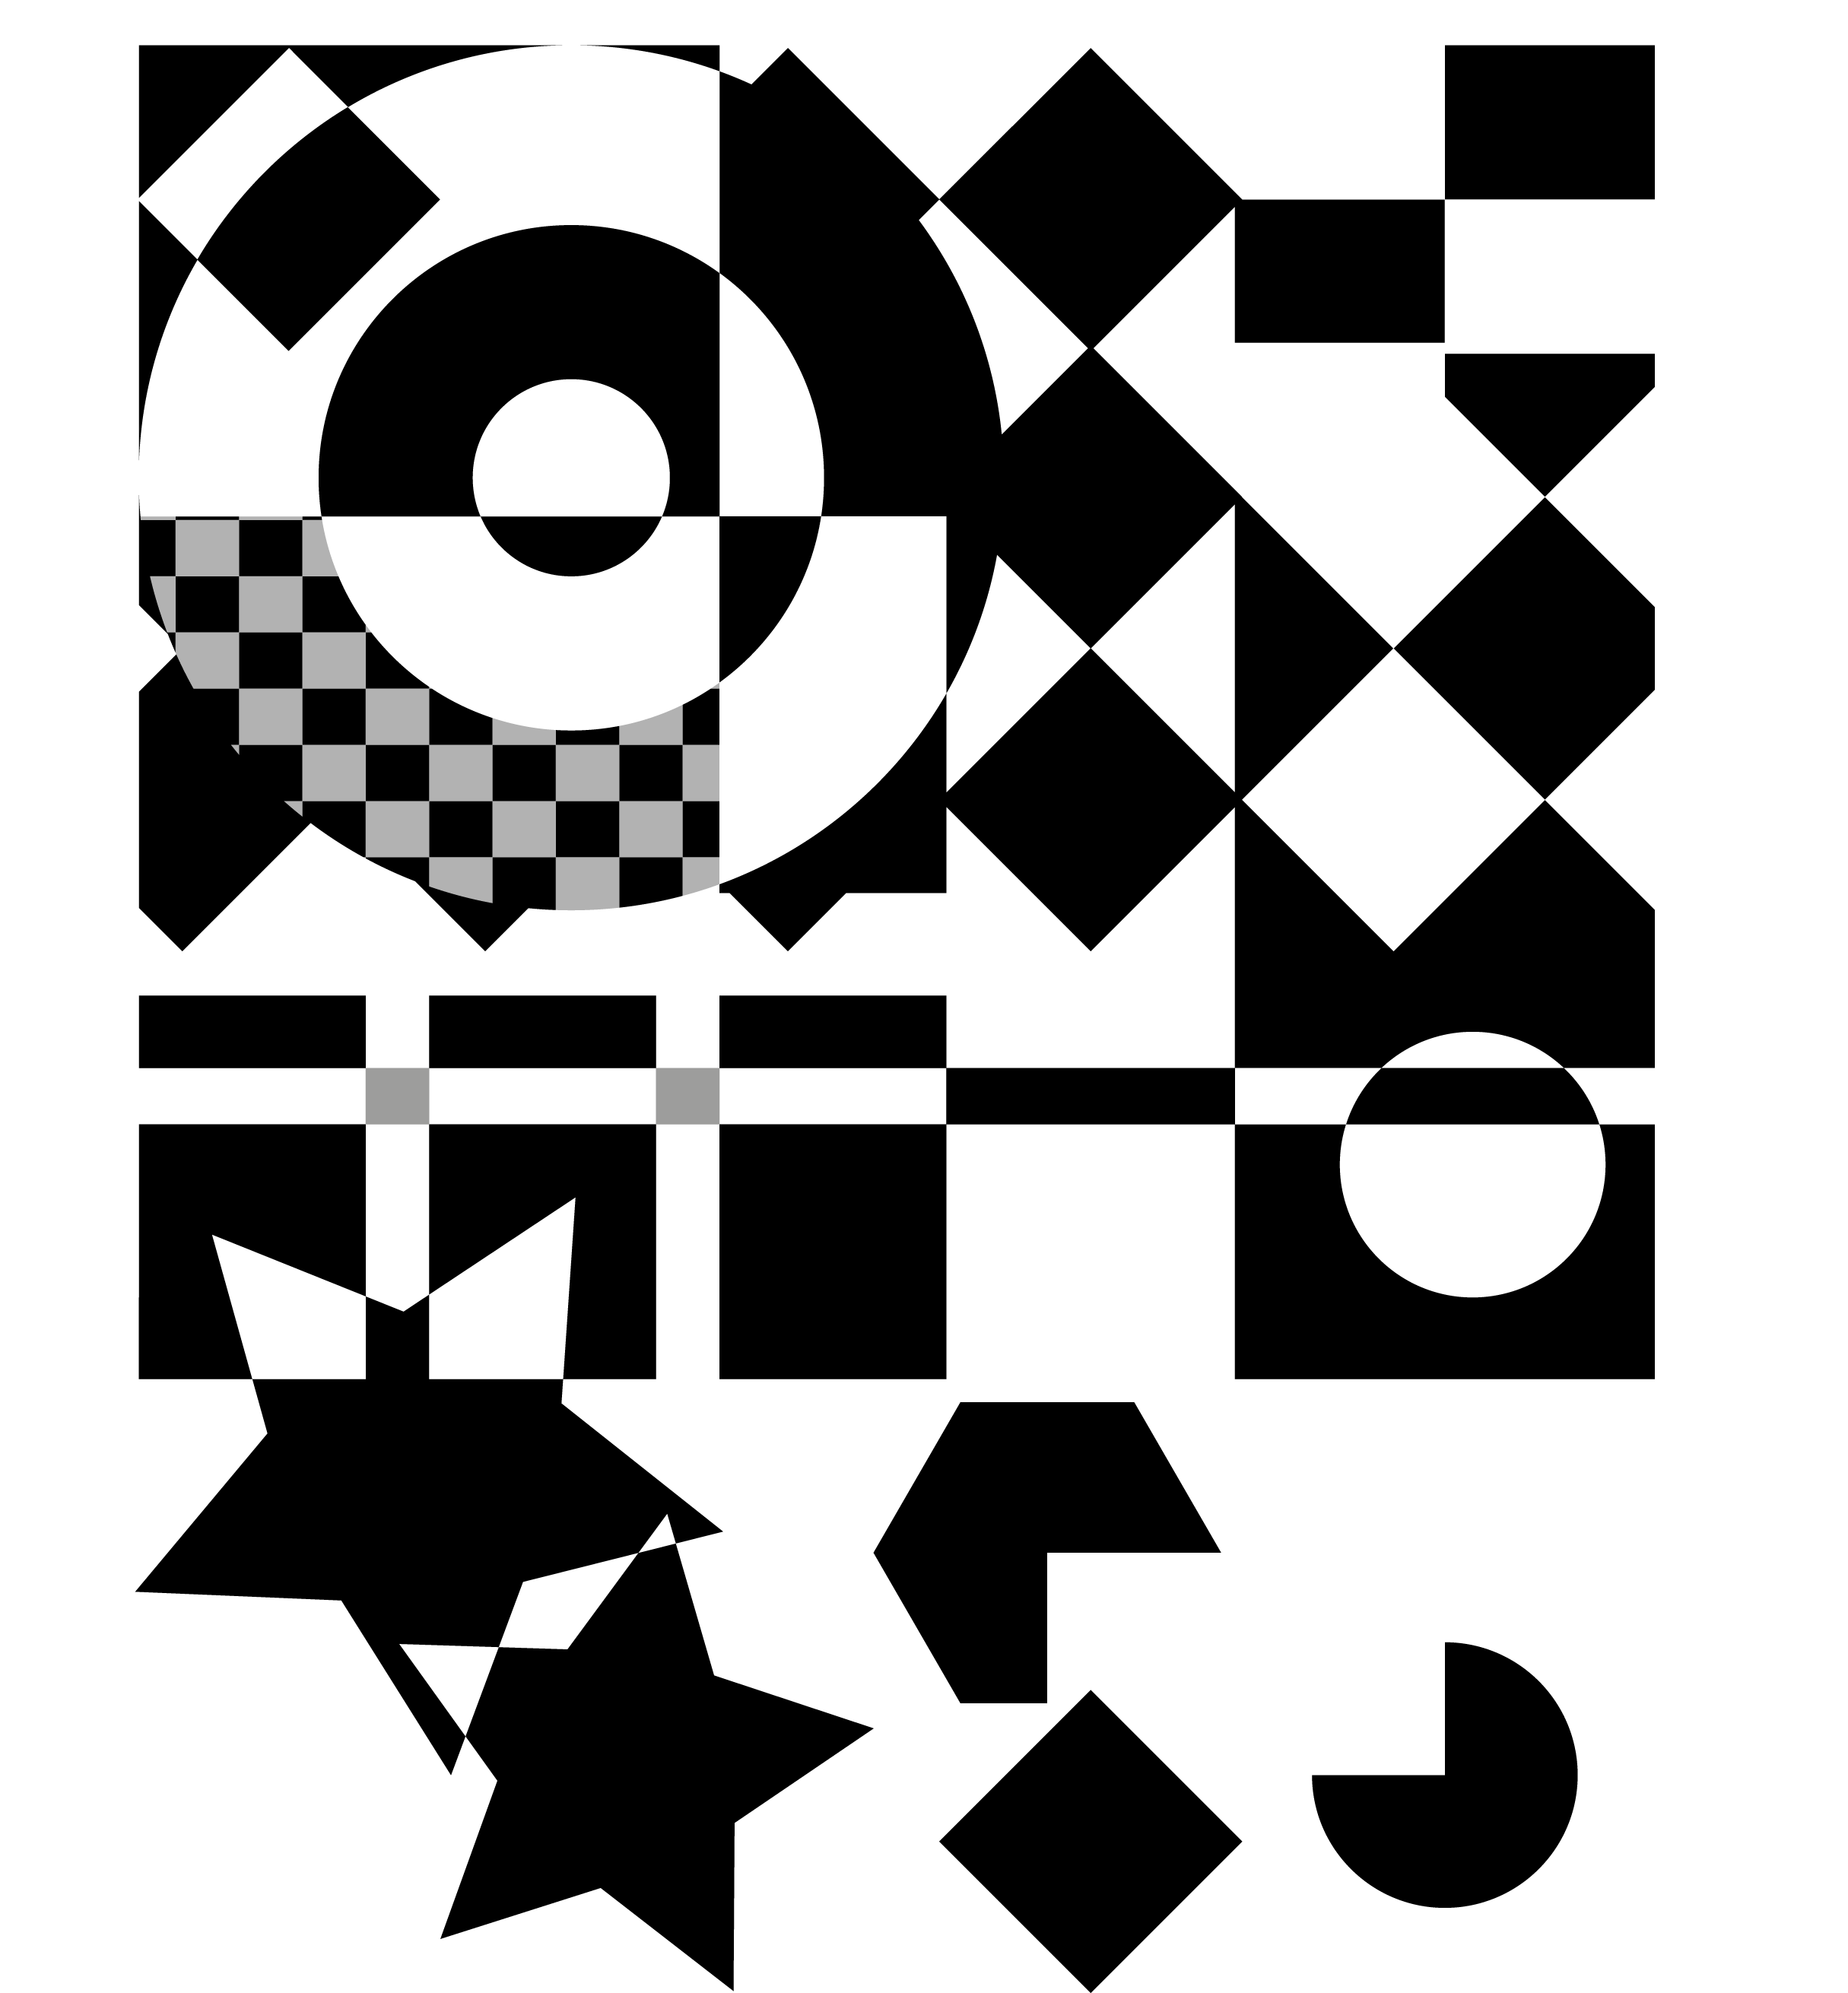
\includegraphics[width=50mm,frame]{target.png}
        }
        \hspace{1mm}
        \subfloat[The target is recognized]{
          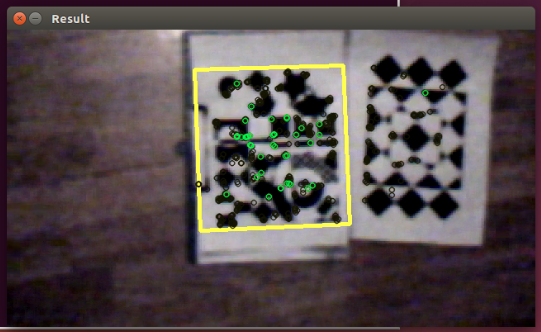
\includegraphics[width=80mm,frame]{target_rec.png}
        }
        \caption{Target and its bounding box found by the ORB algorithm.}
        \label{fig:target}
    \end{figure}

    To recognize the target, a well-known approach called ``feature
    extraction'' is used in this project.
    The idea is that
    it is possible to detect special points on the true image and match them to the points
    detected on a video frame~\cite{FeaturesExplained}.

    There are several algorithms implementing this approach. They are different
    in details, but the general principle is the same.

    In the first stage, features are extracted from an image. It is usual practice
    to use corners as features because it's easy to distinguish
    one corner from another.

    To be able to compare features and to tell one feature from another,
    it is necessary to describe them somehow. That is, a vector of numbers
    called ``descriptor'' is calculated for each feature. Now, if the distance
    between two descriptors is small enough, we can say that we have a match.

    Various algorithms uses various descriptors, but 
    I'm interested in two factors: the descriptors should be scale
    and rotation invariant so that the target can be detected
    regardless of the distance to the camera and rotation.

    In the second stage, descriptors are matched to find the target. OpenCV has two methods
    of matching~\cite{MatchingAndHomography}.
    The first one is a simple brute force algorithm.
    The second one is a FLANN-based
    (Fast Library for Approximate Nearest Neighbors) matcher~\cite{FLANN},
    which is more flexible and can work with big amount of features.

    In the third stage, a homography is to be found to project the source image
    onto the detected place. OpenCV has a standard function for this which
    returns a $3\times3$ transformation matrix.

    The result of this actions can be seen in figure~\ref{fig:match}.

    \begin{figure}[htbp]
        \noindent\centering
            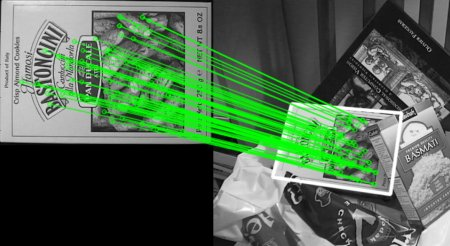
\includegraphics[width=.7\textwidth]{homography_findobj.jpg}
        \caption{Matched features. Source: the OpenCV documentation.}
        \label{fig:match}
    \end{figure}

    \subsection{Features~extraction~algorithms}

    OpenCV has a number of feature extraction algorithms.

    \paragraph{Scale-Invariant Feature Transform}
    SIFT is the first scale-invariant algorithm. It was developed by 
    D. Lowe in 2004~\cite{SIFT, pySIFT}. It uses samples of the same image
    with different sizes (Gaussian pyramid) to detect variously scaled features.
    This makes it work with the large corners as good as with the small ones.

    The descriptors used in this algorithm are vectors of $128$ float values
    representing a brightness histogram of the surrounding area of the feature.

    SIFT consumes a lot of time and memory to process
    due to its $128$-dimentioned descriptors (it takes $512$ bytes
    to store $128$ float values).

    Also, this algorithm is patented and should be purchased to be used.

    \paragraph{Speeded-Up Robust Features}
    SURF was first proposed by H. Bay, T. Tuytelaars, and L. Van Gool
    in 2006~\cite{SURF, pySURF}. This algorithm is an improvement for SIFT.

    SURF is built to use the advantages of ``integral images''.
    It uses different approach for scaling images called ``box filtering''.
    While the Gaussian pyramid needs an image of scale $x$ to calculate the $x+1$,
    ``box filtering'' does not have such limitation.
    Different scales can be calculated in parallel.

    SURF gives a sufficient speed boost but it is still far from the real-time
    performance.

    This algorithm is also patented.

    \paragraph{Features from Accelerated Segment Test}
    FAST is an algorithm brought up by E. Rosten and
    T. Drummond in 2010~\cite{FAST}. It works fast enough to work in
    the real-time applications but it is not robust
    to high levels of noise~\cite{pyFAST}. I've also noted that it generates
    a lot of false-positive matches which slows down the homography estimation.

    \paragraph{Binary Robust Independent Elementary Features}
    BRIEF~\cite{pyBRIEF} is a new method of calculating descriptors.
    It can't extract features so it is often used with other algorithms
    to speed up the descriptors extracting stage.

    \paragraph{Oriented FAST and Rotated BRIEF}
    ORB was proposed by E. Rublee, V. Rabaud, K. Konolige, and Gary R. Bradski
    in 2011. It aims fast descriptor extraction by merging FAST and BRIEF
    algorithms with some improvements.

    It was chosen to be the core of the project because of two reasons.
    First, it is fast and reliable. Second, it's not patented and can be used
    in any application.

    \subsection{Camera~calibration}

    To be able to restore 3d coordinates of the target, it is necessary to
    know target's size and some camera properties, such as the distortion
    coefficients, focal length, optical centers~\cite{OpenCVCalib}.

    The distortion coefficients show how the image is distorted due to 
    the lens imperfection. A typical result of such distortion is shown
    in figure~\ref{fig:calib}.a where the straight lines of the chessboard
    became curved. Another good example of the distortions is a fisheye lens.

    An image can be fixed by mapping pixels
    using five coefficients~\cite{RectificationMatlab}.
    The process of removing the distortion is called ``rectification''.

    % http://www.mathworks.com/help/vision/ug/camera-calibration.html

    \begin{figure}[htbp]
        \noindent\centering
        \subfloat[Distorted image]{
          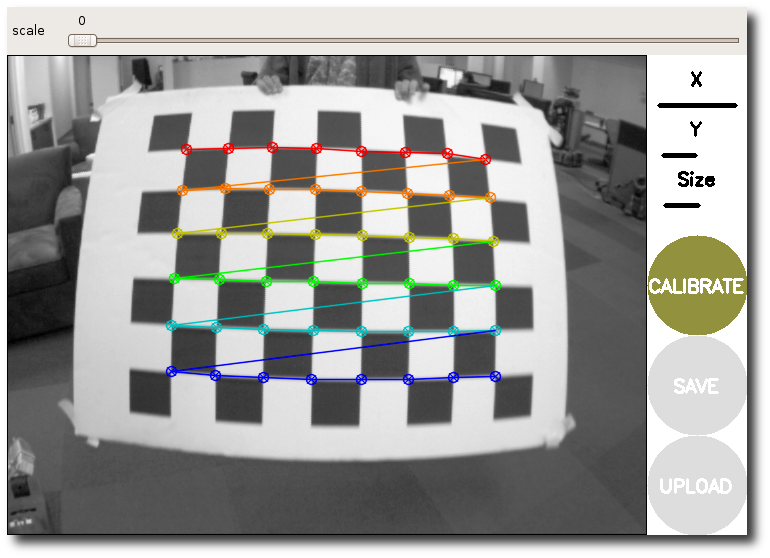
\includegraphics[width=60mm,frame]{calib.png}
        }
        \hspace{1mm}
        \subfloat[Rectified image]{
          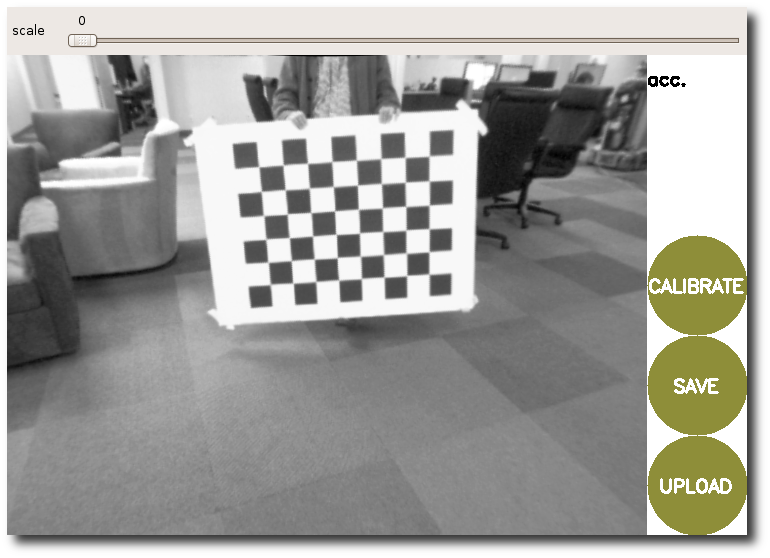
\includegraphics[width=60mm,frame]{calib_fixed.png}
        }
        \caption{Radial image distortion. Source: the ROS site.}
        \label{fig:calib}
    \end{figure}

    The focal length and the optical centers are necessary to
    restore 3d coordinates of the target.

    To get these coefficients, camera needs to be calibrated.
    ROS has a standard tools to do it~\cite{ROSCamCalib} and
    the ArdroneAutonomy supports those tools. That is, you can calibrate the
    camera of your drone and send calibration results to the ArdroneAutonomy driver.
    Than, you can use a standard ``CameraInfo'' ROS topics to get information
    about the camera coefficients in your program.

    \subsection{Target~design}

    The resulting target image is shown in figure \ref{fig:target}.a.
    Its form determined by several factors.
    To reduce errors in the algorithm and increase its performance,
    it's important to follow them.

    The first thing is that the ORB algorithm detects no more than
    a constant number of features
    (300 in this case). Thus, the target image should be complex enough
    to ``draw attantion'' of the algorithm. That is, the majority
    of those 300 features should belong to the tagret.

    The second thing is that features should be well-distributed on the surface
    of the target. If you have all you features in the center, than even
    a slight error would cause homography to be twisted resulting in wobbling.
    However, if you have good distribution of features, matching
    errors will be less influential.

    The third thing is that all corners in the target image should be different
    from each other. ORB uses scale- and rotation-invariant descriptors.
    This means that you have to use different angles for different corners,
    otherwise there will be matching errors. For example, the chessboard
    pattern has very good distribution of features. However, all descriptors
    extracted from those features will be the same so the algorithm will match
    them chaotically.

    And the last one is about what image to use as a true image.

    If you try to find image~\ref{fig:target}.a
    in the image \ref{fig:target}.b, you'll get no match.
    The reason is that the image~\ref{fig:target}.b is small and blurred
    while the image~\ref{fig:target}.a is not. These images have different
    features and different descriptors!

    So, you need to intentionally blur the true image that will be used
    fo find the target. Or you can go even further. You can capture
    you target and than use the result as a true image. For example,
    figure~\ref{fig:target_captured} shows what is used in this project
    as a true image.

    \begin{figure}[htbp]
        \noindent\centering
            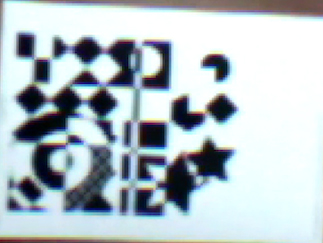
\includegraphics[width=.3\textwidth]{target_captured.jpg}
        \caption{Target image as captured by the bottom camera of the drone.}
        \label{fig:target_captured}
    \end{figure}

    \subsection{Code}

    So, the ORB algorithm is used to detect features and the FLANN-based
    matcher is used to match them.

    The entire procedure is implemented in the controller node.
    
    The code is split into four parts:
    features detection, matching, homography estimation, and 3D coordinates
    estimation.

    First, I extract features and descriptors from the frame. It's done
    by simply calling the ``cv2.ORB()'' extractor.
    I stop the algorithm if there are less than 15 features extracted:

    \begin{lstlisting}[frame=single,language=Python]
image_detect = self.detect(img)

if len(image_detect.kp) < self.min_points:
    return
    \end{lstlisting}

    \begin{lstlisting}[frame=single,language=Python]
def detect(self, img, *args, **kwargs):
    kp, desc = self.detector.detectAndCompute(
        img, None, *args, **kwargs)
    return Detect(kp, desc)
    \end{lstlisting}

    Here, ``self.detector'' is an instance of the ``cv2.ORB'' class and the 
    ``Detect'' class is a simple container which stores features
    and descriptors.

    Second, I match the newly extracted features with those extracted from the
    true image.
    I stop the algorithm if there are less than 15 features matched.

    \begin{lstlisting}[frame=single,language=Python]
def match(self, image_detect):
    # Match the descriptors
    matches = self.matcher.knnMatch(
        # True image descriptors
        self.pattern_detect.desc,
        # Extracted descriptors
        image_detect.desc,
        k=self.knn_parameter)

    # Filter out features that has
    # several possible matches.
    good_matches = [i for i in matches if len(i) == 2]

    # Filter out unreliable matches
    # (that is, only matches that have small distance
    # between the descriptors are used).
    ratio_matches = [m for m, n in good_matches
                     if m.distance <
                     self.match_test_ratio * n.distance]
    
    return ratio_matches
    \end{lstlisting}

    Third, I get the homography matrix using the ``cv2.findHomography()'' function.

    At this stage, another check happens. To be sure that there are no
    false-positive matches, I check that the bounding box of the target
    is actually a rectangle.

    Fourth, I get the 3d coordinate using the ``cv2.solvePnPRansac()'' function.

    So, as the output, I get the 3d coordinates of the target
    in the coordinate frame relative of camera.

    \section{Drone~control~algorithm}
    \label{sec:drone_control_algorithm}

    The second part of the control application is the control algorithm
    itself.

    After the image was processed, I need to generate commands for the drone.
    It is done in a very simple manner: the coordinates of the target are
    transformed to the coordinate frame which stays constant relatively
    to the world. Than, a new velocity for the drone is calculated
    as a function from that vector.

    \subsection{Drone's~position~and~coordinate~transformation}

    \begin{figure}[htbp]
        \noindent\centering
            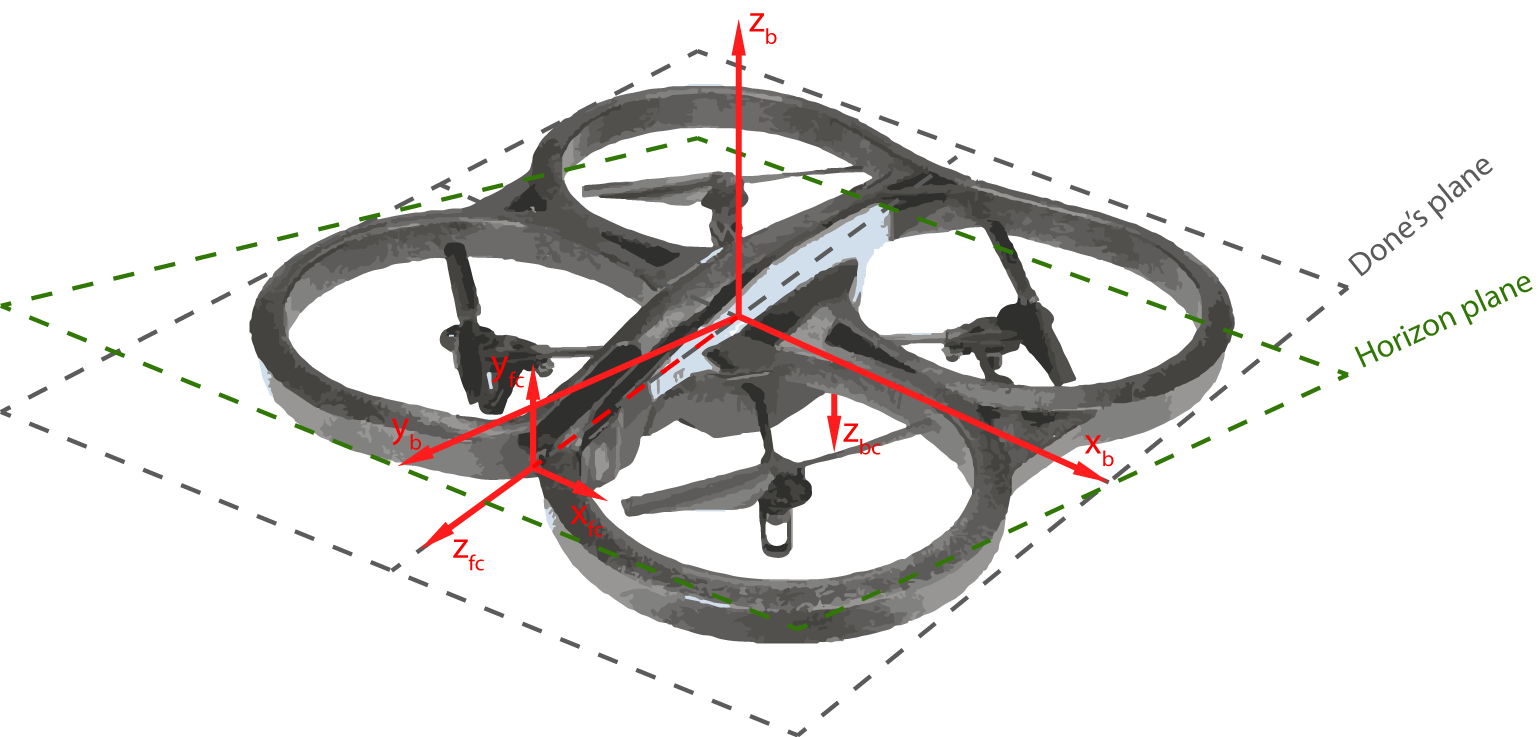
\includegraphics{frames.png}
        \caption{Drone's base frame $x_b, y_b, z_b$, front camera frame $x_{fc}, y_{fc}, z_{fc}$, bottom camera frame $x_{bc}, y_{bc}, z_{bc}$.}
        \label{fig:frames}
    \end{figure}

    ROS provides a very convenient tool for tracking position of
    objects. This tool is called ``tf'' (from ``transform'').

    It tracks position and rotation of coordinate frames over the time and allows
    to transform coordinates from one frame to another.

    ArdroneAutonomy publishes four frames.
    Thee of them are displayed in figure~\ref{fig:frames}.
    The front and the bottom camera frames are sticked to the drone's cameras.
    The odometry base frame has its origin in the center of the drone, but its
    rotation remains constant relatively to the world.
    The fourth frame is not displayed in the figure. In ideal world with
    no measurement errors, it would be stuck to the drone's
    launch position.

    \subsection{Controlling~the~drone}

    So, the output of a computer vision part is the coordinates of the target
    in the coordinate system of the bottom camera. I need to transform them
    to be in the base coordinate system. It is done by multiplying
    the coordinate vector by a transform matrix which comes from ``tf'':

    \begin{lstlisting}[frame=single,language=Python]
def get_rot_matrix(self):
    # names of the coordinate frames
    frm = 'ardrone/ardrone_base_bottomcam'
    to = 'ardrone/odom'

    # Wait for the next update of the transform matrix
    self.tf.waitForTransform(
        frm, to, rospy.Time(0), rospy.Duration(3))
    # Request the matrix
    trans, rot = self.tf.lookupTransform(
        frm, to, rospy.Time(0))

    # Correct axis direction
    # by converting a quaternion to Euler angles
    # and changing their signs.
    x, y, z = euler_from_quaternion(rot)
    return np.array(euler_matrix(-x, -y, z)), rot
    \end{lstlisting}

    Now I can multiply coordinates by the matrix:

    \begin{lstlisting}[frame=single,language=Python]
rot_matrix, rot_quaternion = self.get_rot_matrix()
point = coordinates.dot(rot_matrix)
    \end{lstlisting}

    However, it's not finished yet: the $y$ axis of the base coordinate frame
    always points to the same direction and I need it to point to the
    forward direction of the drone. Thus, I rotate the coordinate vector
    using the Euler angles extracted from the matrix:

    \begin{lstlisting}[frame=single,language=Python]
yaw = euler_from_quaternion(rot_quaternion, axes='szxy')[0]
x, y, z = point[0][0], point[0][1], point[0][2]
x, y = x * cos(yaw) - y * sin(yaw), x * sin(yaw) + y * cos(yaw)
    \end{lstlisting}

    Now I can send a new command to the drone:

    \begin{lstlisting}[frame=single,language=Python]
left = (min(max(x, -700), 700) / 1000)
forward = -(min(max(y - 50, -700), 700) / 1000)
self.controller.send_vel(forward, left)
    \end{lstlisting}

    And, of course, if no target is found, I make the drone to auto-hover:

    \begin{lstlisting}[frame=single,language=Python]
self.controller.hover()
    \end{lstlisting}

    \section{Conslusion}

    The algorithm works normally assuming that no external forces,
    such as wind, applied to the drone. Due to the small field of view
    of the camera, the drone cannot follow the target longer than
    a few minutes.

    However, the main goal is achieved. The reusable code is presented
    which makes writing of applications for the ArDrone 2 easier and faster.

    \newpage

    \setcounter{page}{1}
    \pagenumbering{roman}

    \begin{thebibliography}{9}

\bibitem{ArdroneAuthonomy}
Ardrone Authonomy repository and documentation is currently available at \\
http://www.ardrone-autonomy.readthedocs.org/en/latest/ \\
https://github.com/AutonomyLab/ardrone\_autonomy

\bibitem{ROSsite}
ROS documentation is currently available at \\
http://www.wiki.ros.org

\bibitem{rostopic}
Rostopic is a tool for displaying debug information about ROS Topics.
Its documentation is currently available at \\
http://www.wiki.ros.org/rostopic

\bibitem{SURF}
Herbert Bay, Andreas Ess, Tinne Tuytelaars, Luc Van Gool, \emph{Speeded Up Robust Features},
ETH Zurich, Katholieke Universiteit Leuven

\bibitem{ORB}
Ethan Rublee, Vincent Rabaud, Kurt Konolige, Gary Bradski, \emph{ORB: an efficient alternative to SIFT or SURF},
Willow Garage, Menlo Park, California

\bibitem{OpenCVCalib}
OpenCV calibration tool is explained at \\
http://docs.opencv.org/2.4/doc/tutorials/calib3d/\\
camera\_calibration/camera\_calibration.html

\bibitem{OpenCV3dRec}
OpenCV 3d reconstruction tool is explained at \\
http://docs.opencv.org/2.4/modules/calib3d/doc/\\
camera\_calibration\_and\_3d\_reconstruction.html

\bibitem{roslaunch}
Roslaunch is a tool for launching ROS application.
Its documentation is currently available at \\
http://wiki.ros.org/roslaunch

\bibitem{FeaturesExplained}
A good explanation on how features work is available at \\
http://opencv-python-tutroals.readthedocs.io/en/latest/\\
py\_tutorials/py\_feature2d/py\_features\_meaning/py\_features\_meaning.html

\bibitem{MatchingAndHomography}
The documentation on the features matching process in OpenCV is available at \\
http://opencv-python-tutroals.readthedocs.io/en/latest/\\
py\_tutorials/py\_feature2d/py\_matcher/py\_matcher.html

\bibitem{FLANN}
Marius Muja, David G. Lowe, \emph{Fast Approximate Nearest Neighbors with Automatic Algorithm Configuration}, 2009

\bibitem{SIFT}
D. Lowe, \emph{Distinctive Image Features from Scale-Invariant Keypoints},
University of British Columbia, 2004

\bibitem{pySIFT}
http://opencv-python-tutroals.readthedocs.io/en/latest/py\\
\_tutorials/py\_feature2d/py\_sift\_intro/py\_sift\_intro.html

\bibitem{pySURF}
http://opencv-python-tutroals.readthedocs.io/en/latest/\\
py\_tutorials/py\_feature2d/py\_surf\_intro/py\_surf\_intro.html

\bibitem{FAST}
Edward Rosten, Tom Drummond, \emph{Machine learning for high-speed corner detection}, 2006

\bibitem{pyFAST}
http://opencv-python-tutroals.readthedocs.io/en/latest/\\
py\_tutorials/py\_feature2d/py\_fast/py\_fast.html

\bibitem{pyBRIEF}
http://opencv-python-tutroals.readthedocs.io/en/latest/\\
py\_tutorials/py\_feature2d/py\_brief/py\_brief.html

\bibitem{RectificationMatlab}
http://www.mathworks.com/help/vision/ug/camera-calibration.html

\bibitem{ROSCamCalib}
Documentation for the camera calibration tool for ROS is available at \\
http://wiki.ros.org/camera\_calibration


    \end{thebibliography}

\end{document}
